% Construction : deux piles côte à côte, entrée à gauche (x = -2.4), sortie à
%   droite (x = 1.6), largeur 1.6, socle en y = 0, éléments d'épaisseur 0.55.
%   Entrée empilée d, c, b de bas en haut ; sortie vide ; flèche de bascule.
% SVG : x = 150 + 34x, y = 122 - 34y.
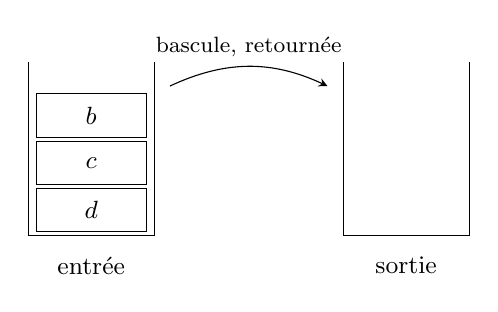
\begin{tikzpicture}[scale=1, >=stealth, every node/.style={font=\small}]
  \draw (-3.2, 0) -- (-1.6, 0) -- (-1.6, 2.2); \draw (-3.2, 0) -- (-3.2, 2.2);
  \draw (0.8, 0) -- (2.4, 0) -- (2.4, 2.2); \draw (0.8, 0) -- (0.8, 2.2);
  \foreach \e/\y in {d/0.05, c/0.65, b/1.25}
    \draw (-3.1, \y) rectangle node {$\e$} (-1.7, \y+0.55);
  \draw[->] (-1.4, 1.9) to[bend left=25] (0.6, 1.9);
  \node[above, font=\footnotesize] at (-0.4, 2.15) {bascule, retournée};
  \node[below] at (-2.4, -0.15) {entrée};
  \node[below] at (1.6, -0.15) {sortie};
\end{tikzpicture}
